\smalltitle{سوال 4}
\noindent
\begin{latin}
  If both players knew what $\alpha$ was, the question would be quite simple as below.
    %   \begin{istgame}[xscale=2,font=\footnotesize]
    %     \xtdistance{12mm}{16mm}
    %     \istroot(0)[initial node]{A}
    %       \istb{a}[al]
    %       \istb{b}[ar]
    %     \endist
    %     \xtdistance{10mm}{12mm}
    %     \istroot(1a)(0-1)<180>{B}
    %       \istb{c}[al]{0.9}
    %       \istb{d}[ar]{0.7}
    %     \endist
    %     \istroot(1b)(0-2)<0>{C}
    %       \istb{e}[al]{0.4}
    %       \istb{f}[ar]{0.6}
    %       \xtShowEndPoints[oval node]
    %     \endist
    %     \istroot(2a)(1a-2)<0>{C}
    %     %   \istb{e}[al]{0.4}
    %     %   \istb{f}[ar]{0.6}
    %       \xtShowEndPoints[oval node]
    %     \endist
    %     % \xtdistance{10mm}{12mm}
    %     % \istroot(2a)(1a-1)<0>{LLD}
    %     %   \istb{t}[al]{0.4}
    %     %   \istb{j}[ar]{0.6}
    %     %   \xtShowEndPoints[oval node]
    %     % \xtInfoset[](1a)(2a)
    %   \end{istgame}
    %   \\\\
    \begin{center}
        

      \begin{istgame}[xscale=2,font=\footnotesize]
        \xtdistance{15mm}{45mm}
        \istroot(0)[initial node]{}
          \istb{0.5,\alpha=1}[al]
          \istb{0.5,\alpha=-1}[ar]
        \endist
        \xtdistance{18mm}{15mm}
        \istroot(1a)(0-1)<180>{P1}
          \istb{1}[]{}
          \istb{2}[]{}
          \istb{4}[]{}
        \endist
        \istroot(1b)(0-2)<0>{P1}
        \istb{1}[]{}
        \istb{2}[]{}
        \istb{4}[]{}
        %   \xtShowEndPoints[oval node]
        \endist
        \xtdistance{22mm}{5mm}
        \istroot(2a)(1a-1)<180>{P2}
        \istb{1}[]{(1,-1)}
        \istb{2}[]{(2,-2)}
        \istb{4}[]{(4,-4)}
        %   \istb{e}[al]{0.4}
        %   \istb{f}[ar]{0.6}
          \xtShowEndPoints[oval node]
        \endist
        \istroot(2b)(1a-2)<0>{P2}
        \istb{1}[]{(2,-2)}
        \istb{2}[]{(4,-4)}
        \istb{4}[]{(8,-8)}
        %   \istb{e}[al]{0.4}
        %   \istb{f}[ar]{0.6}
          \xtShowEndPoints[oval node]
        \endist
        \istroot(2c)(1a-3)<0>{P2}
        \istb{1}[]{(4,-4)}
        \istb{2}[]{(8,-8)}
        \istb{4}[]{(16,-16)}
        %   \istb{e}[al]{0.4}
        %   \istb{f}[ar]{0.6}
          \xtShowEndPoints[oval node]
        \endist
        \istroot(2d)(1b-1)<180>{P2}
        \istb{1}[]{(-1,1)}
        \istb{2}[]{(-2,2)}
        \istb{4}[]{(-4,4)}
        %   \istb{e}[al]{0.4}
        %   \istb{f}[ar]{0.6}
          \xtShowEndPoints[oval node]
        \endist
        \istroot(2e)(1b-2)<0>{P2}
        \istb{1}[]{(-2,2)}
        \istb{2}[]{(-4,4)}
        \istb{4}[]{(-8,8)}
        %   \istb{e}[al]{0.4}
        %   \istb{f}[ar]{0.6}
          \xtShowEndPoints[oval node]
        \endist
        \istroot(2f)(1b-3)<0>{P2}
        \istb{1}[]{(-4,4)}
        \istb{2}[]{(-8,8)}
        \istb{4}[]{(-16,16)}
        %   \istb{e}[al]{0.4}
        %   \istb{f}[ar]{0.6}
          \xtShowEndPoints[oval node]
        \endist
        % \xtInfoset[](1a)(1b)
      \end{istgame}
    \end{center}
    if : 
    $
    \begin{cases}
            \alpha = 1  \rightarrow 
               & x:1,y:2 = x:2,y:1 ,, x:1,y:4=x:2,y:2=x:4,y:1,,x:2,y:4 = x:4,y:2
               \\[1ex]
            \alpha = -1  \rightarrow 
               & x:1,y:2 = x:2,y:1 ,, x:1,y:4=x:2,y:2=x:4,y:1,,x:2,y:4 = x:4,y:2
    \end{cases}
    $
    \\\\\\
    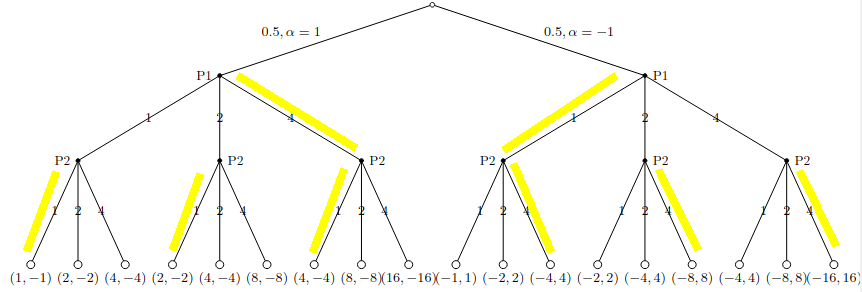
\includegraphics[scale=0.5]{q4.png}
    \\
    As you could see the best strategies for each player if they each knew about $\alpha$ would be : \\
    $
    \begin{cases}
            \alpha = 1  \rightarrow 
               & x:4, y:1
               \\[1ex]
            \alpha = -1  \rightarrow 
               & x:1, y:4
    \end{cases}
    $ \\ \\ 
    Now if player 2 \textbf{doesn't know the value of $\alpha$}, he would not know what branch player 1 picked but he know 2 facts, first of all player 1 would never choose 2 and second, player 2 will either choose from (4,-4) (8,-8) (16,-16) or (-1,1) (-2,2) (-4,4) so it would be rational for 
    player 2 to pick the option with best mean value.\\\\
    player 2 : 
    $
    \begin{cases}
      1 \rightarrow 
         & (-4 + 1)/2 = -1.5
         \\[1ex]
      2  \rightarrow 
         & (-8 + 2)/2 = -4
         \\[1ex]
      4 \rightarrow
        & (-16 + 4)/2 = -6
\end{cases}
    $
  So player 2 would be better off if he picked choice \textbf{1}
\end{latin}
 